\documentclass[onecolumn]{article}
\usepackage{graphicx}

\begin{document}

\title{Number of visitors -- an accumulation problem}

\author{Arjen Markus}

\maketitle


\subsection*{Introduction}

Consider the following light-weight "demographic" problem: visitors enter and leave
a museum or a fairground or some such pace. They arrive at more or less arbitrary times
and leave after some arbitrary period. Let us assume that "arbitrary" is not so arbitrary.
Instead, for the sake of argument, we see that at ten minutes' intervals one person enters
and then stays for one hour. These numbers are chosen so that it is easy to draw a graph,
the red line indicating the total number:

\begin{figure}[h]
\begin{center}
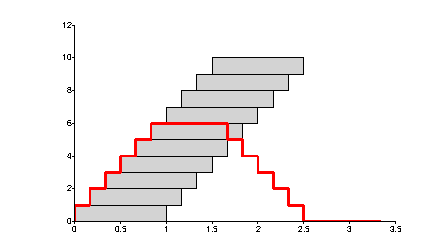
\includegraphics[width=0.7\textwidth]{number_visitors_rough.pdf}
\label{visitorsRough}
\end{center}
\end{figure}

In this particularly simple case the maximum number of people, $N$ is:

\begin{equation}
     N = duration~of~visit~/~interval~of~arrival = 60 / 10 = 6
\end{equation}

The next step is to make this more general:
\begin{itemize}
\item
The number of people that enter is a function $\phi(t)$ of time.
\item
Instead of a fixed contribution of 1 per person, the contribution is an arbitrary function $\lambda(t)$ of the
time since arrival. This makes it possible to consider other problems than merely the number of visitors
over time, for instance a release of a radioactive substance in a lake.
\end{itemize}

So, at time $t$ we have contributions from arrivals up to $t$. The number/amount of arrivals at a time $\tau \leq t$
is $\phi(\tau)$ and since they have been around for a time $t-\tau$, the contribution is $\lambda(t-\tau)$.

The total contribution $F(t)$ of all arrivals up to time $t$ is therefore:
\begin{equation}
\label{contribution}
    F(t) = \int^t_{-\infty} \phi(\tau) \lambda(t-\tau) d\tau
\end{equation}

\subsection*{Evaluation of the integral}

Let us take a closer look at our example:
\begin{itemize}
\item
The visitors start coming in at time $t = 0$ and the last one enters at $t = T$. So:
\begin{eqnarray}
            \phi(t) &=& n, ~~~~~~ 0 \leq t \leq T \\
\nonumber           &=& 0, ~~~~~~ \textrm{otherwise}
\end{eqnarray}
\item
The visitors stay for a period P:
\begin{eqnarray}
          \lambda(t) &=& 1, ~~~~~~ 0 \leq t \leq P \\
\nonumber            &=& 0, ~~~~~~ \textrm{otherwise}
\end{eqnarray}
\end{itemize}

These functions can be expressed as a sum of two Heaviside step functions, which makes evaluating the integral
for different periods easier (see the appendix). The result is indeed the function you would expect:

\begin{figure}[h]
\begin{center}
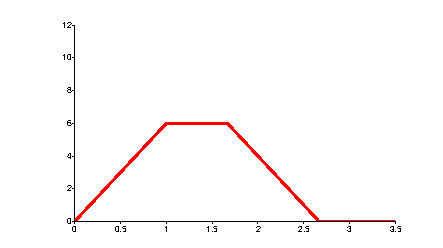
\includegraphics[width=0.7\textwidth]{number_visitors_smooth.pdf}
\label{visitorsSmooth}
\end{center}
\end{figure}

\subsection*{Release of a radioactive substance}

As a second example, consider the continuouns (and constant) release of a radioactive substance in a lake.
We assume that there is no outflow and that the inflow is compensated by evaporation, for simplicity and
to keep the model valid. We further assume that the release has been continuous for much longer than the
half life of the substance, so that:
\begin{eqnarray}
    \phi(t)    &=& M ~~~~~~~~~ \textrm{mass rate} \\
    \lambda(t) &=& e^{-\alpha t} ~~~~~~ \textrm{radioactive decay}
\end{eqnarray}
Then:
\begin{eqnarray}
          F(t) &=& \int^t_{-\infty} M e^{- \alpha (t-\tau)} d\tau          \\
\nonumber      &=& M e^{- \alpha t} \int^t_{-\infty} e^{\alpha \tau} d\tau \\
\nonumber      &=& M / \alpha
\end{eqnarray}


\subsection*{Appendix}
The evaluation of the integral in equation \ref{contribution} with the given functions is easiest by representing the
two functions $\lambda(t)$ and $\phi(t)$ via the Heaviside step function, $\textrm{H}(t)$:
%
\begin{eqnarray}
\nonumber    \phi(t)    &=& n \cdot (\textrm{H}(t) - \textrm{H}(t-T)) \\
\nonumber    \lambda(t) &=& \textrm{H}(t) - \textrm{H}(t-P)
\end{eqnarray}

Filling in these expressions in the integral gives:
\begin{eqnarray}
             F(t) &=& n \int_{-\infty}^t (\textrm{H}(\tau) - \textrm{H}(\tau-T)) \cdot (\textrm{H}(t - \tau) - \textrm{H}(t - \tau-P)) d\tau \\
\nonumber         &=& n \int_{-\infty}^t \Bigl( \textrm{H}(\tau) \cdot (\textrm{H}(t - \tau) - \textrm{H}(\tau) \cdot \textrm{H}(t - \tau - P) \\
\nonumber         & & ~~~~~~~~~~~~ - \textrm{H}(\tau-T) \cdot \textrm{H}(t - \tau) + \textrm{H}(\tau-T) \cdot \textrm{H}(t - \tau-P) \Bigr) d\tau
\end{eqnarray}

Consider the four separate contributions:
\begin{eqnarray}
             F_1(t) &=& \int_{-\infty}^t \textrm{H}(\tau) \cdot \textrm{H}(t-\tau) d\tau \\
\nonumber           &=& \int_0^t \textrm{H}(t-\tau) d\tau
\end{eqnarray}

\noindent resulting in:
\begin{eqnarray}
             F_1(t) &=& \textrm{max} (t, 0)
\end{eqnarray}

The second term:
\begin{eqnarray}
             F_2(t) &=& \int_{-\infty}^t \textrm{H}(\tau) \cdot \textrm{H}(t-\tau-P) d\tau \\
\nonumber           &=& \int_0^t \textrm{H}(t-\tau-P) d\tau     \\
\nonumber           &=& \textrm{max}( t-P, 0)
\end{eqnarray}

The third term:
\begin{eqnarray}
             F_3(t) &=& \int_{-\infty}^t \textrm{H}(\tau-T) \cdot \textrm{H}(t-\tau) d\tau \\
\nonumber           &=& \int_T^t \textrm{H}(t-\tau) d\tau \\
\nonumber           &=& \textrm{max}( t-T, 0)
\end{eqnarray}

The fourth term:
\begin{eqnarray}
             F_4(t) &=& \int_{-\infty}^t \textrm{H}(\tau-T) \cdot \textrm{H}(t-\tau-P) d\tau \\
\nonumber           &=& \int_T^t \textrm{H}(t-P-\tau) d\tau \\
\nonumber           &=& \int_T^{t-P} \textrm{H}(t-P-\tau) d\tau \\
\nonumber           &=& \textrm{max}( t-P-T, 0)
\end{eqnarray}

The end result is:
\begin{eqnarray}
             F(t) &=& n \cdot \Bigl( F_1(t) - F_2(t) - F_3(t) + F_4(t) \Bigr) \\
\nonumber         &=& n \cdot \bigl( \textrm{max}(t,0) - \textrm{max}(t-P,0) - \textrm{max}(t-T,0) + \textrm{max}(t-P-T,0) \bigr)
\end{eqnarray}

This is a piecewise linear function with breakpoints at 0, T, P and P+T.

\end{document}
